\documentclass[11pt, a4paper]{article}
\usepackage[utf8]{inputenc}

\usepackage[margin=1in]{geometry} 
\usepackage{amsmath,amsthm,amssymb}
\usepackage[margin=1in]{geometry} 
\usepackage{amsmath,amsthm,amssymb}

\usepackage[slovene]{babel}
\usepackage{color}
\usepackage{graphicx}
\usepackage{amssymb}
\usepackage{amsmath}
\usepackage{mathtools}
\usepackage{commath}
\usepackage{ragged2e}
\usepackage[T1]{fontenc}
\usepackage[normalem]{ulem}
\usepackage{amsthm}
\usepackage{esvect}
\usepackage{float}
\usepackage{calrsfs}
\DeclareMathAlphabet{\pazocal}{OMS}{zplm}{m}{n}
\newcommand{\Ga}{\mathcal{G}}
\mathtoolsset{showonlyrefs} 

\newcommand\setItemnumber[1]{\setcounter{enumi}{\numexpr#1-1\relax}}


\newtheorem{theorem}{Trditev}[section]
\newtheorem{corollary}{Posledica}[section]
\newtheorem{lemma}[section]{Lema}
\theoremstyle{definition}
\newtheorem{definition}{Definicija}[section]
\theoremstyle{example}
\newtheorem{example}[section]{Primer}
\theoremstyle{izrek}
\newtheorem{izrek}[section]{Izrek}

\begin{document}
\begin{center}
\thispagestyle{empty}
\parskip=14pt%
\vspace*{3\parskip}%
\begin{Huge} Sevanje črnega telesa \end{Huge}

By

Matic Tonin

ID No. (28181098)

Mentor 

(Rok Dolenec)

\rule{7cm}{0.4pt}

Pod okvirom:

FAKULTETE ZA FIZIKO IN MATEMATIKO, LJUBLJANA

1. 4. 2020

\end{center}
\pagebreak
\section{Naloga}
\begin{enumerate}
\item Izmeri odvisnost svetlobnega toka halogene žarnice v razponu od rahlega žarenja
do maksimalne moci. Pri tem meri tudi moc, ki se troši na žarnici, tako da meriš
tok in napetost.
\item Nariši graf celotne izsevane moci kot funkcijo elektricne moci.
\item Doloci elektricno upornost žarnice kot funkcijo temperature.
\item Nariši graf razmerja med – skozi Si okno – prepušcenim in nemotenim svetlobnim
tokom kot funkcijo temperature žarilne nitke.
\end{enumerate}

Kljub temu, da meritve sam nisem izvajal, bom v poročilu navedel, kakšen bi moral biti postopek dela in kako smo dobili določene mertve. \\
\bigskip
\section{Postopek dela}

Najprej, z ohmmetrom izmerimo upornost žarilne nitke na naši žarnici, da bomo kasneje lahko z njo določili odvisnost upornosti od temperature. Nato jo priključimo na merilnik napetosti in toka in preverimo, pri kateri razdalji je najbolj idealno postaviti merilnik sevanja, da nanj ne bo padel prevelik svetlobni tok. Nato spreminjajmo moč žarnice ter si zapisujemo podatke:elektricno moc, tok in napetost na žarnici ter
moc svetlobnega toka. Prve tri podatke odcitamo z merilnika moci (univerzalnega instrumenta),
ki poleg moci v spodnjem delu okenca kaže tudi tok, napetost in fazni zamik
med obema.
Ko opravimo to meritev, damo pred naš detekor manjši zastor silicija ter ponovimo meritev v istem intervalu. 


\section{Meritve}
\subsection{Meritev pred segrevanjem žarnice}
Še preden začnemo vso meritev najprej izmerimo, koliko je temperatura v sobi in predpostavimo, da ima žarilna nitka žarnice isto temperaturo.

$$T_{zraka}=T_{light}=22.2 C°+/- 0.2C° $$

Nato izmerimo, koliko je upornost žarnice, če čez njo spustimo tok, preden se nitka segreje in dobimo, da je: 

$$R_{light}=121.4 \Omega +/- 0.1 \Omega $$

Nato še izmerimo, kolikšen je začetni svetlobni tok, ki pride do naše aparature za merjenje in si ga zapišemo.

$$P_0=0.5 mW \pm 0.01 mW$$
 
Če to storimo še za silicijevim oknom:
 
$$P_{S0}=0.49 mW \pm 0.01 mW$$

Nato nastavimo še bolometer na razdaljo, ki nam najbolj ustreza in sami smo izbrali, da je: 
$$l=22 mm \pm 2 mm$$

\pagebreak
Če te začetne podatke zberemo v tabelo, dobimo:
\begin{table}[h]

	\begin{tabular}{|c|c|c|c|c|}
		\hline
		\hline
		$T_{light}$ & $R_{light}$ & $P_0$ & $P_{S0}$ & l \\
		\hline
		22.2 C°$\pm$0.2°C & $121.4 \Omega \pm 0.1 \Omega$ & 0.5 mW$\pm$0.01 mW & 0.49 mW$\pm$0.01 mW & 22 mm$\pm$2 mm \\
		\hline
	\end{tabular}
	\caption{Začetni podatki za žarnico}		\label{osnove}
\end{table}

Sedaj začnemo z meritvijo, kjer počasi povečujemo moč na žarnici ter si vse zapisujemo v naši tabeli.
Zaradi prevelike tabele, ki so nam jo posredovali profesorji, bom v mojem poročilu navedel zgolj sliko tabele, samo zato, da vemo, s katerimi podatki operiramo. 

\begin{figure}[htp]
    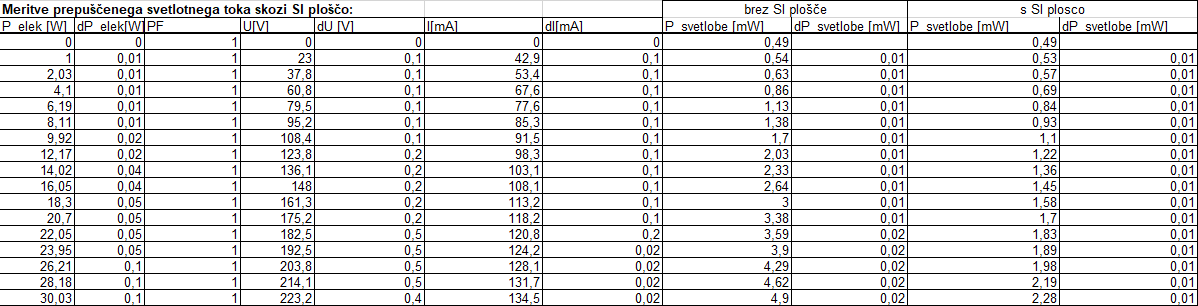
\includegraphics[width=15cm]{Tabela.png}
    \caption{Tabela meritev ki so jih opravili asistenti,}
\end{figure}
\subsection{Graf celotne izsevane moči kot funkcija električne moči}
Da bi narisali graf izsevane moči v odvisntost od električne moči, moramo pogledati, katere podatke imamo. Vidimo, da smo merili električno moč, torej vse kar potrebujemo je celotna izsevana moč.

Vemo, da naš detektor zazna moč $P_{bol}$. Vemo tudi, da nam iz ozadja in okolice prihaja svetlobni tok $P_0$. Ker vemo, kolikšna je površina bolometra, lahko izračunamo, kolikšen je svetlobni tok:
$$j_{bol}=\frac{P_{bol}-P_0}{S_{bol}}$$


Ker vemo, da se nam ohranja moč, po celem izsevanem volumnu, lahko rečemo, da je:
$$P_{izsevan}=j_{bol}*S$$
Kjer je S površina sfere, po kateri potuje svetloba.\\

Če si predstavljamo sfero po kateri potuje svetloba, vidimo, da v resnici naš bolometer zajame zgolj majhen delec cele sfere. Tako zazna zgolj nek delec izsevanega svetlobnega toka in ne celotne sfere. 
\begin{figure}[H]
	\centering
    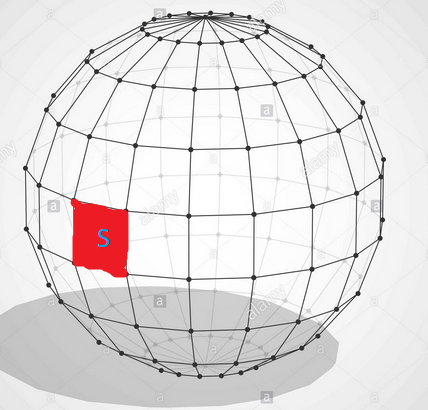
\includegraphics[width=5cm]{Krogla.png}
    \caption{Prikaz širjenja svetlobnega toka, z rdečo je označeno okno detektorja}
\end{figure}

\pagebreak
Torej, če sedaj oba izraza sestavimo skupaj, je izsevan tok kar enak:

$$P_{izsevan}=\frac{P_{bol}-P_0}{S_{bol}}\cdot 4\pi l^2$$

Preprosto rečeno si lahko to formulo razlagamo tudi kot, da je izsevana moč enaka zaznani moči, pomnoženim z razmerjem, koliko sfere zavzame naš detektor.

Sedaj lahko naše vrednosti nanesemo na graf:

\begin{figure}[H]
	\centering
    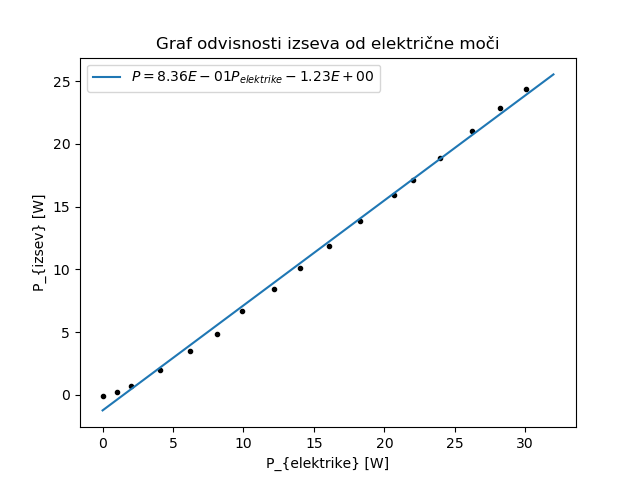
\includegraphics[width=12cm]{Izsev-elektrika.png}
    \caption{Graf odvisnosti izseva od električne moči}
\end{figure}

\pagebreak
\subsection{Graf upora kot funkcija temperature}
Za električno upornost žarnice kot funkcijo temperature smo najprej morali določiti upornost na žarnici. To smo dobili iz preproste zveze, da je

$$R=\frac{U}{I}$$

Te dve obe količini pa smo merili, torej lahko upor za vsako meritev izračunamo.\\
 
Ostane nam samo še izračun temperature v vsaki točki. Ker temperature žarilne nitke nismo merili, si bomo morali pomagati z Stefanovim zakonom. 
 
$$\frac{P}{S}=\int_{0}^{\infty}j(\mu, T)d\mu=\sigma T^4$$

Ker vemo začetne pogoje za žarnico, lahko za naš primer nastavimo razmerje, ki se bo ohranjalo, neodvisno od P in T. 

$$\frac{P}{P_0}=\left(\frac{T}{T_0}\right)^4$$

Kjer sta $T_0$ in $P_0$ temperatura in moč, ki smo ju izmerili na začetku merjenja, podana v tabeli (\ref{osnove})

Sledi, da je temperatura v vsakem trenutku enaka: 

$$T=T_0\sqrt[4]{\frac{P}{P_0}}$$

Tako lahko narišemo graf za vsako meritev.
\begin{figure}[H]
	\centering
    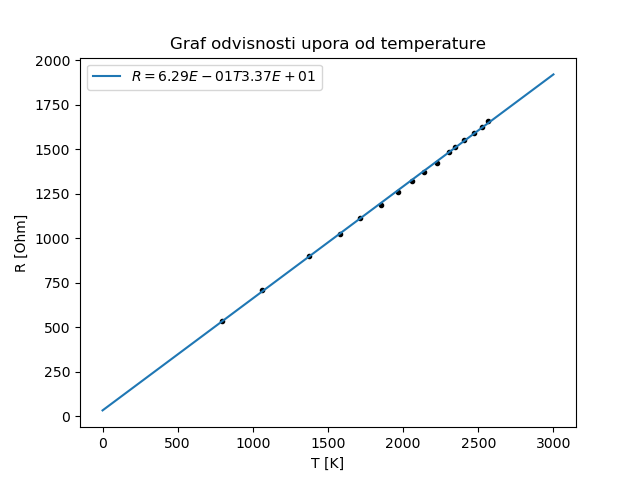
\includegraphics[width=12cm]{Upor-Temperatura.png}
    \caption{Graf odvisnosti upornosti od temperature}
\end{figure}


Če navedemo koeficient v tabelo dobimo: 

\begin{table}[h]
	\centering
	\begin{tabular}{|c|c|c|}
		
		\hline
		Kakšna je bila meritev & Enačba premice & Koeficienta [$\frac{\Omega}{K}$]\\ [0.5ex] 
		\hline
		\hline
		Brez zastora & $R= 0.629 \cdot T +3.37E+01$ &$0.629 \cdot T$ \\
		\hline
		
	\end{tabular}
	\caption{Prikaz koeficientov naše funkcije upora v odvisnosti od temperature}	
\end{table}

\pagebreak
\subsection{Razmerje med celotnim in prepuščenim svetlobnim tokom v odvisnosti od temperature}

Pri tem delu naloge smo dali med naš detektor še silicijevo plast, ki je blokirala del spektra svetlobe. Prav zato pa nam ne velja več Štefanov zakon v celoti, ampak moramo gledati zgolj določen odsek tega integrala. In za naš primer, ko so temperature manjše od 3000K je dobra aproksimacija prepuščenega toka kar: 

$$\frac{P(T)}{P}=1-\frac{15}{\pi^{4}}\left[-y^{3} \log \left(1-e^{-y}\right)+\left(6+6 y+3 y^{2}\right) e^{-y}\right]+O\left(e^{-y}\right), \quad y=\frac{1.1 \mathrm{eV}}{k T}$$

Zakaj je taka enačba je napisano v dodatnih navodilih za izvajanje vaje. \\

Vemo pa tudi, da se po prepustnost toka upadala z večanjem temperature, saj se porazdelitev svetlobe premika izven našega opazovanega okna. Razlaga za to se skriva v Wienovem zakonu, ki nam pove, da se porazdelitev sevanja črnega telesa s spremembo temperature spremeni. V našem primeru, ko višamo temperaturo, se bo ta razlezla in ker imamo pred našim bolometrom silicijevo zaslonko, bo pri neki temperaturi naš spekter ušel izven našega opazovalnega okna.
 
\begin{figure}[H]
	\centering
    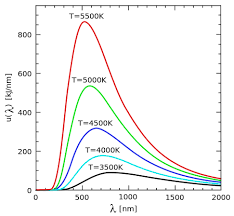
\includegraphics[width=10cm]{Wienov zakon.png}
    \caption{Prikaz spreminjanja porazdelitve oddane svetlobe s spremembo temperature}
\end{figure}
    
Hkrati pa moramo upoštevati tudi popravek zaradi odbojev svetlobe na obeh površinah. V dodatku za obdelavo meritev imamo napisano, da je tako v približku naš faktor tranzmisivnosti kar enak: 

$$T_{plošča}=\frac{2n}{1+n^2}$$

Torej, da bi upoštevali tudi to napako, pomnožimo naše razmerje še s tem faktorjem, da izvemo, koliko toka se izgubi. \\

Če sedaj narišemo naše razmerje dobimo, da je:\\
\bigskip

\begin{figure}[H]
	\centering
    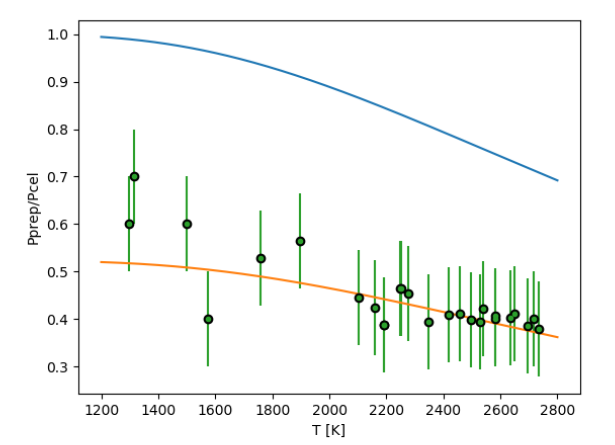
\includegraphics[width=10cm]{Graf,Silicij.png}
    \caption{Graf razmerja moči v odvisnosti od temperature. Modra krivulja je
teoretičen približek brez popravka, oranžna je približek z popravkom, točke
pa so izmerki z mero napake}
\end{figure}

\pagebreak
\section{Napake meritev in rezultati}
Za določene meritve smo že navedli napake, manjkajo pa nam še nekatere napake in zbrani podatki rešitev.
\subsection{Graf celotne izsevane moči kot funkcije električne moči}

Pri tej meritvi se pojavi kar nekaj napak in sicer:
\begin{enumerate}
\item \underline{Napaka meritve ploskve detektorja}: \\
Kot prvo se nam pojavi napaka meritve detektorja, ki jo ocenimo na: $\delta S_{bol}=\frac{0.0025{cm}^2}{1{cm}^2}$. Torej da smo se pri meritvi kvadratnega centimetra zmotili za 0.05cm v eno in 0.05 v drugo smer, kar je 0.0025.
Kar lahko zanemarimo, saj je manjše od procenta. 
\item \underline{Napaka meritve razdalje}:\\
Druga napaka ki se pojavi, se pojavi zaradi merjenja oddaljenosti detektorja od žarilne nitke. Naša ocena je $\delta l=\frac{0.2}{30}$, kar je ponovno manjše kot procent (0.66\%).
Tudi to lahko zanemarimo v končni fazi.
\item \underline{Napaka fitanja grafa in koeficienta premice}:  \\
Pri tem delu pa se napaka fitanja premice večinsko odraža kar v natančnosti meritve moči na senzorju.
Zanjo smo izračunali da je približno 7.5\%.
\end{enumerate}
Sedaj, ko smo navedli vse napake, vidimo, da znašajo okoli 8\%, torej lahko zapišemo rezultat:

$$\underline{\underline{P_{izsev}=(0.836 \pm 0.0668)\cdot P_{elektrike}}}$$

\subsection{Graf upora kot funkcija temperature}
Prav tako moramo tu upoštevati kar nekaj napak:
\begin{enumerate}
\item \underline{Napaka meritev napetosti in toka}:\\
Vidimo, da se nam pri merjenju upora pojavita dve napaki in sicer pri meritvi toka in pri meritvi napetosti. Te dve napaki se nato pokažeta pri računanju koeficienta premice za naš upor. 
\item \underline{Napak meritve začente moči in temperature}: \\
Te dve napaki smo že navedli v osnovnih podatkih in vemo njune vrednosti, ponovno pa se bosta odražali v koeficientu, le da napaka začetne moči, ker je pod 4 korenom ne bo tako močno vplivala. Da navedemo njune vrednosti: $\delta T=0.009$ in $\delta P_0= 0.02$, ampak ker je pod 4 korenom, jo pri računanju temperature še delimo s štiri, torej bo njen končni vpliv na temperaturo enak 0.005.
\item \underline{Napaka meritve celotne moči}:\\
Napaka celotne moči je bila izračunana že prej in je v resnici kar podana kot celotna napaka koeficienta grafa, torej je približno 8 \%. Ampak ker je tudi ta pod 4-korenom, se deli s 4 in dobimo le 2\%.
\item \underline{Napaka fitanja grafa}: \\
Pri tem delu se napaka fitanja pojavi kot skupek vseh napak ki smo jih zgoraj navedli, predvsem zaradi napake upora. Ko jo zračunamo, dobimo okoli 6\%.
\end{enumerate}

Po seštevku vseh napak vidimo,da je naš celoten rezultat enak:

$$\underline{\underline{R(T)=(0.629 \pm 0.059 )\frac{\Omega}{K}\cdot T}}$$

\subsection{Razmerje med celotnim in prepuščenim svetlobnim tokom v odvisnosti od temperature}
Napake tega dela meritve pa so: 
\begin{enumerate}
\item \underline{Napaka meritve temperature}: \\
Napako meritve temperature smo napisali že pri prejšnji meritvi in je enaka kar napaki vrednosti koeficienta na grafu, če mu odštejemo napako upora, ki je približno 3\%.
Torej je napaka te meritve okoli 6\%.
\item \underline{Napaka fitanja}: \\
Vidimo, da smo imeli pri tem delu kar zahteven izraz za fitanje na krivuljo, saj je vseboval veliko matematičnih operacij. Zato se je vrednost napake spreminjala in na koncu smo jo izračunali, da je okoli 12 \%.
\end{enumerate}
Skupna napaka znaša torej okoli 15 \%, kar je razvidno tudi na spodnji sliki. \\
\bigskip

\begin{figure}[H]
	\centering
    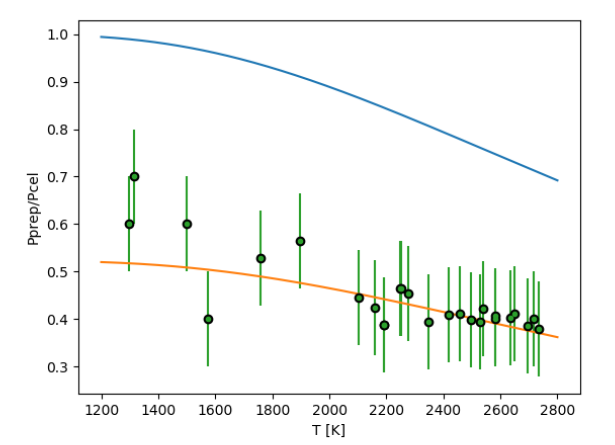
\includegraphics[width=10cm]{Graf,Silicij.png}
    \caption{Graf razmerja moči v odvisnosti od temperature. Modra krivulja je
teoretičen približek brez popravka, oranžna je približek z popravkom, točke
pa so izmerki z mero napake}
\end{figure}

\end{document}